\section{Análisis y Desarrollo}

  Se presenta un análisis descriptivo de los datos recolectados sobre el rendimiento académico de los estudiantes de la UTP en relación con el uso de herramientas de inteligencia artificial. Se calculan de acuerdo a los temas vistos en clase.

  % Pregunta 1 - Género
  \subsection{Género de la muestra:}
  
  \textbf{Tabla de frecuencias:}
  
  El siguiente cuadro muestra la distribución de género de los participantes en la muestra, dividiéndose en masculino y femenino, así mismo se muestra la frecuencua absoluta, acumulada, relativa porcentual y relativa porcentual acumulada.

  \begin{multicols}{2}
    \begin{enumerate}
      \item \begin{center}
        \textbf{Marca de Clase: $x_i$}
        \hrulefill
        \begin{equation*}
            x_i = \dfrac{L_i + L_s}{2}
        \end{equation*}
    \end{center}
    \vspace{-0.5cm}
    Donde:
    \begin{itemize}
        \item $L_i$: Límite inferior de la clase.
        \item $L_s$: Límite superior de la clase.
    \end{itemize}
    Para este caso, la marca de clase para valores cualitativos es el valor mismo por lo que $x_1 = Masculino$ y $x_2 = Femenino$.

    \item \begin{center}
        \textbf{Frecuencia Absoluta: $f_i$}
        \hrulefill
        \begin{equation*}
          f_i = \sum_{i=1}^{n} x_i
        \end{equation*}
    \end{center}
    \vspace{-0.7cm}
    Donde:
    \begin{itemize}
        \item $x_i$: Marca de clase.
        \item $f_i$: Frecuencia absoluta.
    \end{itemize}
    Para este caso, $f_1 = 51$ y $f_2 = 26$.

    \item \begin{center}
      \textbf{Frecuencia Acumulada: $F_i$}
      \hrulefill
      \begin{equation*}
        F_i = \sum_{i=1}^{n} f_i
      \end{equation*}
    \end{center}
    \vspace{-0.5cm}
    Donde:
    \begin{itemize}
        \item $f_i$: Frecuencia absoluta.
        \item $F_i$: Frecuencia acumulada.
    \end{itemize}

    \item \begin{center}
      \textbf{Frecuencia Relativa \%: $h_i\%$}
      \hrulefill
      \begin{equation*}
        h_i = \dfrac{f_i}{n} \times 100
      \end{equation*}
    \end{center}
    \vspace{-1cm}
    Donde:
    \begin{itemize}
        \item $f_i$: Frecuencia absoluta.
        \item $h_i$: Frecuencia relativa porcentual.
    \end{itemize}

    \item \begin{center}
      \textbf{Frecuencia Acumulada \%: $H_i\%$}
      \hrulefill
      \begin{equation*}
        H_i = \sum_{i=1}^{n} h_i
      \end{equation*}
    \end{center}
    \vspace{-1cm}
    Donde:
    \begin{itemize}
        \item $h_i$: Frecuencia relativa porcentual.
        \item $H_i$: Frecuencia acumulada porcentual.
    \end{itemize}
    \end{enumerate}
  \end{multicols}
  \vspace{-0.5cm}
  Finalmente se muestra la tabla de frecuencias:

  \renewcommand{\arraystretch}{1.5} % Ajusta la altura de las filas
\begin{table}[ht]
    \centering
    \begin{tabular}{l @{\hskip 0.5cm} c @{\hskip 0.5cm} c @{\hskip 0.5cm} c @{\hskip 0.5cm} c}
      \hline
      \textbf{Género} & \textbf{$f_i$} & \textbf{$F_i$} & \textbf{$h_i$ (\%)} & \textbf{$H_i$ (\%)} \\ \hline
      Masculino       & 51             & 51             & 66.23               & 66.23               \\ \hline
      Femenino        & 26             & 77             & 33.77               & 100.00              \\ \hline
      Total           & 77             &                & 100.00              &                     \\
    \end{tabular}
    \caption{Distribución por género con frecuencias absolutas, acumuladas y relativas.}
    \label{tab:genero-frecuencias}
\end{table}

\textbf{Interpretación de resultados:}

La tabla de frecuencias muestra que el 66.23\% de los participantes en la muestra son de género masculino, mientras que el 33.77\% son de género femenino. La distribución de género en la muestra refleja una mayor representación de estudiantes masculinos en comparación con las estudiantes femeninas.

  % Pregunta 2 - Carrera
  \subsection{Carrera a la que pertenecen los estudiantes:}

A continuación se muestra un cuadro con los datos de cualitativos de las carreras de los estudiantes pertenecientes a muestra, se pretender hacer una ordenación de los mismos, generar una tabla de frecuencias y establecer una gráfica representativa.

\begin{table}[H]
  \centering
  \hspace*{-2cm} % Mueve la primera tabla más a la izquierda
  \begin{minipage}{0.35\textwidth} % Ajustar el ancho según sea necesario
    \centering
    \begin{tabular}{l @{\hskip 0.6cm} l}
      \hline
      \textbf{Carrera} & \textbf{Acrónimo} \\ \hline
      Ingeniería       & \small{ING}                \\ \hline
      Psicología       & \small{PSI}                \\ \hline
      Comunicaciones   & \small{COM}                \\ \hline
      Arquitectura     & \small{ARQ}                \\ \hline
      Derecho          & \small{DER}                \\ \hline
      Administración   & \small{ADM}                \\ \hline
      Negocios         & \small{NEG}                \\ \hline
      Medicina         & \small{MED}                \\ \hline
      Gastronomía      & \small{GAS}               \\ \hline
    \end{tabular}
    \caption{Carreras y acrónimos de los estudiantes en la muestra.}
    \label{tab:carreras-acronimos}
  \end{minipage}
  \hspace{0.2cm} % Espacio horizontal entre las tablas
  \begin{minipage}{0.45\textwidth} % Ajustar el ancho según sea necesario
    \centering
    \caption{Representación de Carreras}
    \begin{tabular}{|>{\scriptsize}m{0.6cm}|>{\scriptsize}m{0.6cm}|>{\scriptsize}m{0.6cm}|>{\scriptsize}m{0.6cm}|>{\scriptsize}m{0.6cm}|>{\scriptsize}m{0.6cm}|>{\scriptsize}m{0.6cm}|>{\scriptsize}m{0.6cm}|>{\scriptsize}m{0.6cm}|>{\scriptsize}m{0.6cm}|} \hline \scriptsize{\textbf{ING}} & \scriptsize{\textbf{ING}} & \scriptsize{\textbf{ING}} & \scriptsize{\textbf{ING}} & \scriptsize{\textbf{ING}} & \scriptsize{\textbf{ING}} & \scriptsize{\textbf{ING}} & \scriptsize{\textbf{ING}} & \scriptsize{\textbf{ING}} & \scriptsize{\textbf{ING}} \\ \hline \scriptsize{\textbf{ING}} & \scriptsize{\textbf{ING}} & \scriptsize{\textbf{ING}} & \scriptsize{\textbf{ING}} & \scriptsize{\textbf{ING}} & \scriptsize{\textbf{ING}} & \scriptsize{\textbf{ING}} & \scriptsize{\textbf{ING}} & \scriptsize{\textbf{ING}} & \scriptsize{\textbf{ING}} \\ \hline \scriptsize{\textbf{ING}} & \scriptsize{\textbf{ING}} & \scriptsize{\textbf{ING}} & \scriptsize{\textbf{ING}} & \scriptsize{\textbf{ING}} & \scriptsize{\textbf{ING}} & \scriptsize{\textbf{ING}} & \scriptsize{\textbf{ING}} & \scriptsize{\textbf{ING}} & \scriptsize{\textbf{ING}} \\ \hline \scriptsize{\textbf{ING}} & \scriptsize{\textbf{ING}} & \scriptsize{\textbf{ING}} & \scriptsize{\textbf{ING}} & \scriptsize{\textbf{ING}} & \scriptsize{\textbf{ING}} & \scriptsize{\textbf{ING}} & \scriptsize{\textbf{ING}} & \scriptsize{\textbf{ING}} & \scriptsize{\textbf{ING}} \\ \hline \scriptsize{\textbf{ING}} & \scriptsize{\textbf{ING}} & \scriptsize{\textbf{ING}} & \scriptsize{\textbf{ING}} & \scriptsize{\textbf{ING}} & \scriptsize{\textbf{DER}} & \scriptsize{\textbf{DER}} & \scriptsize{\textbf{DER}} & \scriptsize{\textbf{PSI}} & \scriptsize{\textbf{PSI}} \\ \hline \scriptsize{\textbf{PSI}} & \scriptsize{\textbf{PSI}} & \scriptsize{\textbf{PSI}} & \scriptsize{\textbf{MED}} & \scriptsize{\textbf{COM}} & \scriptsize{\textbf{ARQ}} & \scriptsize{\textbf{ARQ}} & \scriptsize{\textbf{ADM}} & \scriptsize{\textbf{ADM}} & \scriptsize{\textbf{ADM}} \\ \hline \scriptsize{\textbf{ADM}} & \scriptsize{\textbf{NEG}} & \scriptsize{\textbf{NEG}} & \scriptsize{\textbf{NEG}} & \scriptsize{\textbf{NEG}} & \scriptsize{\textbf{NEG}} & \scriptsize{\textbf{GAS}} & & & \\ \hline \end{tabular}
  \end{minipage}
\end{table}

\textbf{Tabla de frecuencias:}

El siguiente cuadro muestra la distribución de carreras de los participantes en la muestra, dividiéndose en las diferentes opciones de carrera, así mismo se muestra la frecuencia absoluta, acumulada, relativa porcentual y relativa porcentual acumulada.

% Tenemos estos datos:

% Ing: 55
% Der: 3
% Psi: 5
% Med: 1
% Com: 1
% Arq: 2
% Adm: 4
% Neg: 5
% Gast: 1

\begin{table}[H]
  \centering
  \begin{tabular}{l @{\hskip 0.6cm} c @{\hskip 0.6cm} c @{\hskip 0.6cm} c @{\hskip 0.6cm} c}
    \hline
    \textbf{Carrera} & \textbf{$f_i$} & \textbf{$F_i$} & \textbf{$h_i$ (\%)} & \textbf{$H_i$ (\%)} \\ \hline
    Ingeniería       & 55             & 55             & 71.43               & 71.43               \\ \hline
    Derecho          & 3              & 58             & 3.90                & 75.32               \\ \hline
    Psicología       & 5              & 63             & 6.49                & 81.82               \\ \hline
    Medicina         & 1              & 64             & 1.30                & 83.12               \\ \hline
    Comunicaciones   & 1              & 65             & 1.30                & 84.42               \\ \hline
    Arquitectura     & 2              & 67             & 2.60                & 87.01               \\ \hline
    Administración   & 4              & 71             & 5.19                & 92.21               \\ \hline
    Negocios         & 5              & 76             & 6.49                & 98.70               \\ \hline
    Gastronomía      & 1              & 77             & 1.30                & 100.00              \\ \hline
    Total            & 77             &                & 100.00              &                     \\ \hline
  \end{tabular}
  \caption{Distribución de Carreras de los Estudiantes en la Muestra.}
  \label{tab:carreras-frecuencias}
\end{table}

\newpage

\textbf{Gráfico estadístico:}

A continuación se muestra un gráfico de barras que representa la distribución de carreras de los estudiantes en la muestra, permitiendo visualizar la cantidad de participantes por cada opción de carrera.

\begin{figure}[H]
  \centering
  \begin{tikzpicture}
      \begin{axis}[
          width=0.8\textwidth, % Ancho del gráfico
          height=0.5\textheight, % Altura del gráfico
          xlabel={Carrera}, % Etiqueta del eje X
          ylabel={Frecuencia Absoluta}, % Etiqueta del eje Y
          xtick=data, % Ticks del eje X
          ytick={0, 10, 20, 30, 40, 50, 60}, % Ticks del eje Y
          ymin=0, % Límite inferior del eje Y
          ymax=60, % Límite superior del eje Y
          bar width=0.6cm, % Ancho de las barras
          enlarge x limits=0.15, % Ampliar límites en el eje X
          ylabel near ticks, % Posicionar la etiqueta del eje Y cerca de los ticks
          xlabel near ticks, % Posicionar la etiqueta del eje X cerca de los ticks
          grid=major, % Mostrar la cuadrícula
          title={Distribución de Carreras de los Estudiantes en la Muestra}, % Título del gráfico
          xticklabel style={align=center}, % Alinear los ticks del eje X
          symbolic x coords={ING, DER, PSI, MED, COM, ARQ, ADM, NEG, GAS}, % Etiquetas del eje X
      ]
          \addplot[
              ybar,
              color=blue % Color de las barras
          ] 
          coordinates {(ING, 55) (DER, 3) (PSI, 5) (MED, 1) (COM, 1) (ARQ, 2) (ADM, 4) (NEG, 5) (GAS, 1)};
      \end{axis}
  \end{tikzpicture}
  \caption{Distribución de Carreras de los Estudiantes en la Muestra.}
  \label{fig:carreras-frecuencias}
\end{figure}

\textbf{Interpretación de resultados:}

La tabla de frecuencias y el gráfico de barras muestran que la mayoría de los participantes en la muestra pertenecen a la carrera de Ingeniería, con un 71.43\% de representación, seguida por Negocios con un 6.49\% y Psicología con un 6.49\%. Las carreras de Medicina, Comunicaciones y Gastronomía tienen la menor representación en la muestra, con un 1.30\% cada una.
  
  % Pregunta 3 -  Edad
  \newpage
  \subsection{Edades de los encuestados}
	\noindent \textbf{Tabla de Frecuencias:} \\ \\
	Tabla que refleja las distribución de las respuestas de los encuestados ante los rangos de edades proporciados en la encuesta; muestra a su vez la frecuencia absoluta, frecuencia absoluta acumulada, frecuencia relativa(porcentual) y frecuencia relativa(porcentual) acumulada.
	
	%3ra pregunta del cuestionario, tabla de edades
	\begin{table}[h!]
		\centering
		\renewcommand{\arraystretch}{1.5} % Adjust this value to increase spacing
		\begin{tabular}{l c c c c}
			\hline
			{Rango de edad} & {\(f_i\)} & \textit{Fi} & \textit{hi}(\%) & \textit{Hi}(\%)\\
			\hline
			19 años o menos   & 39 & 39 & 50.65\% & 50.65\%\\
			20 - 23 años       & 20 & 59 & 25.97\% & 76.62\%\\
			24 - 27 años       & 8  & 67 & 10.39\% & 87.01\%\\
			28 años o más      & 10 & 77 & 12.99\% & 100\%\\
			\hline
			Total			   & 77 & & 100\% \\
			\hline
		\end{tabular}
		\caption{Distribución de respuestas por rango de edad}
		\label{tabla:edad}
	\end{table}
	% Formula y solución de la media(promedio)
	\noindent \textbf{Media (\(\overline{X}\))}: \\
	Para el rango "19 años o menos" se ha tomado como referencia 17.5
	\begin{equation*}
		\overline{X} = \frac{\sum (x_i \cdot f_i)}{\sum f_i} = \frac{(17.5 \cdot 39) + (21.5 \cdot 20) + (25.5 \cdot 8) + (30 \cdot 10)}{77} \approx 20.99
	\end{equation*}\\
	
	% Formula y solución de la mediana
	\noindent \textbf{Mediana}: \\ 
	La mediana es el valor que divide el conjunto de datos en dos partes iguales. Con \(N = 77\), la mediana se encuentra en la posición:
	\begin{equation*}
		\text{Posición de la mediana} = \frac{N + 1}{2} = \frac{77 + 1}{2} = 39
	\end{equation*}
	Por lo tanto, la mediana corresponde a "Menos de 19 años".\\
	
	% Solución de la moda
	\noindent \textbf{Moda}: \\ 
	La moda es el valor con la mayor frecuencia, que en este caso es Menos de 19 años con \(f_i = 39\). \\ \\
	
	\newpage
	\noindent\textbf{Gráfico de Tendencia Central}
	\begin{figure}[H]
		\centering
		\hspace*{-1.5cm}
		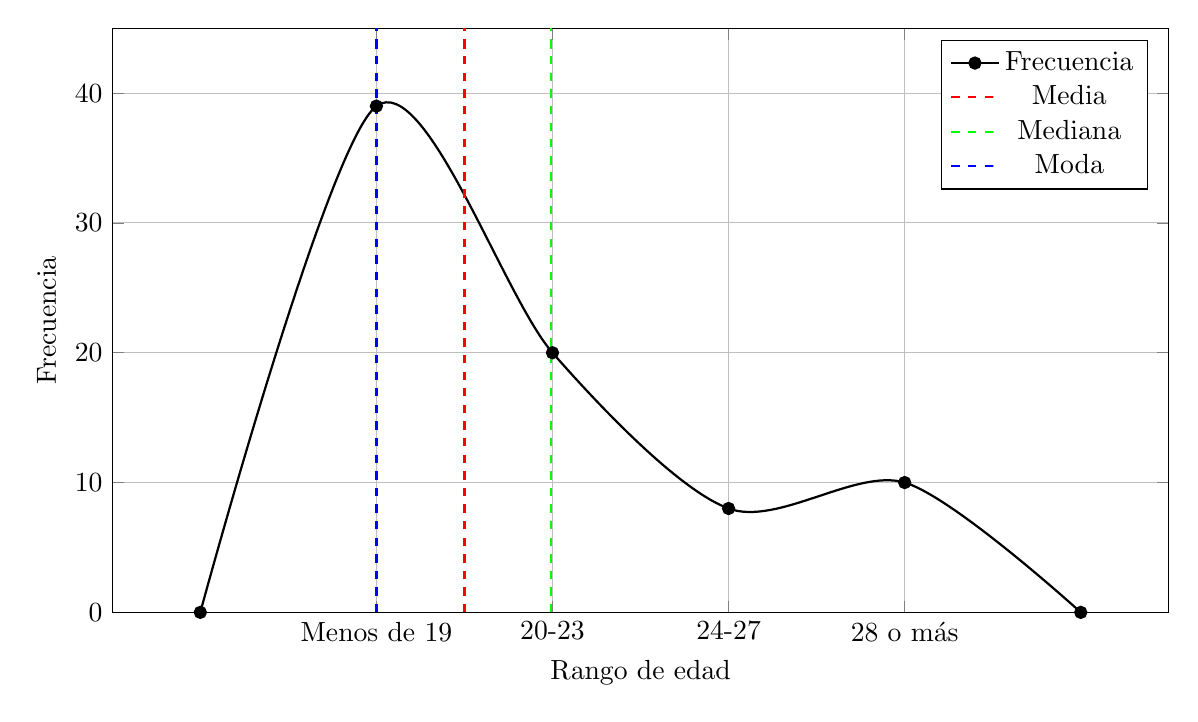
\begin{tikzpicture}
			\begin{axis}[
				width=15cm, height=9cm,
				xlabel={Rango de edad},
				ylabel={Frecuencia},
				xtick={1,2,3,4},
				xticklabels={Menos de 19, 20-23, 24-27, 28 o más},
				extra x ticks={1.5, 1.99},
				ymin=0, ymax=45,
				grid=major,
				smooth,
				tension=0.5,
				extra tick style={opacity=0} %Invisibiliza los ticks extra declarados
				]
				
				% Poligono de frecuencias
				\addplot[
				mark=*,
				color=black,
				thick
				] coordinates {
					(0,0)
					(1,39) % Menos de 19 años
					(2,20) % 20-23
					(3,8)  % 24-27
					(4,10) % 28 o más
					(5,0)
				};
				
				%Media
				\addplot[
				color=red,
				thick,
				dashed
				] coordinates {(1.5, 0) (1.5, 45)}; 
				%Mediana
				\addplot[
				color=green,
				thick,
				dashed
				] coordinates {(1.99, 0) (1.99, 45)};
				%Moda
				\addplot[
				color=blue,
				thick,
				dashed
				] coordinates {(1, 0) (1, 45)}; 
				\legend{Frecuencia, Media, Mediana, Moda}
			\end{axis}
		\end{tikzpicture}
		\caption{Gráfico de frecuencia con línea de tendencia}
	\end{figure}
	\begin{center}
		\noindent Interpretación: Se puede apreciar que la concentración de las edades está alrededor del rango de "menos de 19 años" dado que tanto la moda como la media pertenecen a este rango
	\end{center}
  
  % Pregunta 14
  \newpage
  \subsection{Empleo en horas a la semana de las I.A.}
\textbf{Tabla de Frecuencias:} \\

\begin{table}[h!]
	\centering
	\renewcommand{\arraystretch}{1.5} 
	\begin{tabular}{l c c c }
		\hline
		{Rango de horas} & {\(f_i\)} & \textit{\(h_i\)}(\%) & \textit{\(x_i\)}\\
		\hline
		Menos de una hora	& 42 & \(55.26\%\) & \(0.5\)	\\
		1 - 5 horas			& 26 & \(34.21\%\) & \(3\)		\\
		6 - 10 horas 		& 6  & \(7.89\%\)  & \(8\)		\\
		11 - 20 horas 		& 2  & \(2.63\%\)  & \(15.5\)	\\
		Más de 20 horas		& 0  & \(0\%\)     & \(23\)		\\
		\hline
		Total				& 76 & \(100\%\) \\
		\hline
	\end{tabular}
	\caption{Empleo de las inteligencias artificiales en horas a la semana}
	\label{tabla:EmpleoEnHoras}
\end{table}

\textbf{Media(\(\bar{x}\)):}
\begin{equation*}
	\bar{x} = \frac{(0.5 \times 42) + (3 \times 26) + (8 \times 6) + (15.5 \times 2) + (23 \times 0)}{76} \approx 2.34
\end{equation*}
La media semanal del uso de las herramientas de inteligencia artificial es de 2.34 horas, este bajo promedio sugiere que, en general, los encuestados no están profundamente ligados al uso de estas herramientas \\ \\

\noindent\textbf{Varianza:} \\
Se usará varianza muestral.
\begin{equation*}
	s^2 = \frac{(0.5 - 2.34)^2 + (3 - 2.34)^2 + (8 - 2.34)^2 + (15.5 - 2.34)^2 + (23 - 2.34)^2}{75} \approx 8.48
\end{equation*} \\

\begin{minipage}[t]{0.5\textwidth}
	\noindent\textbf{Desviación Estandar:}
	\begin{equation*}
		s = \sqrt{8.48} \approx 2.91
	\end{equation*}
	
\end{minipage}%
\hfill
\begin{minipage}[t]{0.5\textwidth}
	\noindent\textbf{Coeficiente de Variación:}
	\begin{equation*}
		\frac{2.91}{2.34} \times 100 \approx 124.36
	\end{equation*}  
\end{minipage} \\ \\

Las medidas de disperción sugieren que el uso de las herramientas de IA es generalmente bajo entre los encuestados, con una sustancial variabilidad causada por algunos pocos que la usan por extensos periodos de tiempo.
  
  % Pregunta 15
  \newpage
  \subsection{Percepción del Impacto Negativo de la I.A. en el aprendizaje}
\noindent\textbf{Tabla de Frecuencias:}

\begin{table}[h!]
	\centering
	\renewcommand{\arraystretch}{1.5}
	\begin{tabular}{l c c }
		\hline
		Respuestas & \(f_i\) & \(h_i\) \\
		\hline
		Nada & 8 & \(10.53\%\) \\
		Poco & 49 & \(64.47\%\) \\
		De manera significativa & 15 & \(19.74\%\) \\
		Mucho & 4 & \(5.26\%\) \\
		Demasiado & 0 & \(0\%\) \\
		\hline
		Total & 76 & \(100\%\) \\
		\hline
	\end{tabular}
	\caption{Percepción del Impacto Negativo de la I.A. en el aprendizaje}
	\label{tabla:percepciónNegativaEnElAprendizaje}
\end{table}

\noindent\textbf{Moda:} En este caso, es "Poco" puesto que es la respuesta más seleccionada \\ \\
\noindent\textbf{Mediana:} Al tratarse de datos ordinales, la mediana es el punto medio, osea los datos en la posiciones 38 y 39  que tambien pertecen a la respuesta "Poco" \\ \\
\noindent\textbf{Interpretación:} La mayoría de los encuestados considera que el uso de las inteligencias artificiales afecta poco a su aprendizaje
  
  % Pregunta 16
  \newpage
  \subsection{Percepción del porcentaje de tareas automatizadas gracias al uso de herramientas de I.A.}
\noindent\textbf{Tabla de Frecuencias:}
\begin{table}[h!]
	\centering
	\renewcommand{\arraystretch}{1.2}
	\begin{tabular}{l c c c c c}
		\hline
		{Rango de porcentaje} & {\(f_i\)} & \textit{Fi} & \textit{hi}(\%) & \textit{Hi}(\%) & \(x_i\)\\
		\hline
		0\%                  & 3  & 3  & 4.17\%  & 4.17\% & 0\% \\
		1\% - 10\%           & 28 & 31 & 38.89\% & 43.06\% & 5.5\% \\
		11\% - 25\%          & 26 & 57 & 36.11\% & 79.17\% & 18\% \\
		25\% - 50\%          & 10 & 67 & 13.89\% & 93.06\% &37.5\% \\
		Más de un 50\%       & 4  & 71 & 5.56\%  & 100\% & 75\% \\
		\hline
		Total                & 71 &    & 100\%   & & \\
		\hline
	\end{tabular}
	\caption{Distribución de respuestas por porcentaje de tareas automatizadas}
	\label{tabla:porcentaje_IA}
\end{table} \\

\noindent\textbf{Media($\bar{x}$):}
\begin{equation*}
	\frac{(3 \times 0\%) + (5.5 \times 28) + (18 \times 26) + (37.5 \times 10) + (75 \times 4)}{71} \approx 18.268\%
\end{equation*}

\noindent\textbf{Varianza:}
\begin{equation*}
	\frac{(0-18.268)^2 + (5.5-18.268)^2 + (18-18.268)^2 + (37.5 - 18.268)^2 + (75 - 18.268)^2}{70} \approx 58.36
\end{equation*}

\begin{multicols}{2}
	\noindent\textbf{Mediana(\(M_e\)):}
	\begin{center}
		$11\% + 14(\frac{35.5 - 31}{26}) \approx 13.42\%$
	\end{center}
	\columnbreak
	\vfill
	\noindent\textbf{Desviación Estandar}
	\begin{center}
		$\sqrt{58.36^2} \approx 7.64$
	\end{center}
\end{multicols}

\noindent\textbf{Percentiles:} Se calculan los percentiles para calcular el coeficiente de asimetría de Pearson

\begin{multicols}{2}
	\noindent$P_{75} = 11\% + 14\left(\frac{53.25 - 31}{26}\right) \approx 22.98\%$ \\ \\
	$P_{25} = 1\% + 9\left(\frac{17.75 - 3}{28}\right) \approx 5.74\%$
	\columnbreak
	\vfill
	\noindent$P_{90} = 25\% + 25\left(\frac{63.9 - 57}{10}\right) \approx 42.25\%$ \\ \\
	$P_{10} = 1\% + 9\left(\frac{7.1 - 3}{28}\right) \approx 2.32\%$
\end{multicols}

\begin{multicols}{2}
	\noindent\textbf{Pearson:} La distribución tiene asimetría positiva
	\begin{equation*}
		3\left(\frac{18.268-13.42}{7.64}\right) \approx 1.90
	\end{equation*}
	\vfill
	\columnbreak
	\noindent\textbf{Curtosis:} La distribución es leptocúrtica
	\begin{equation*}
		\frac{22.98-5.74}{42.25-2.32} \approx 0.43
	\end{equation*}
\end{multicols}

\newpage

\noindent\textbf{Gráfico de medidas de forma}
\begin{figure}[h!]
	\centering
	\hspace*{-1.2cm}
	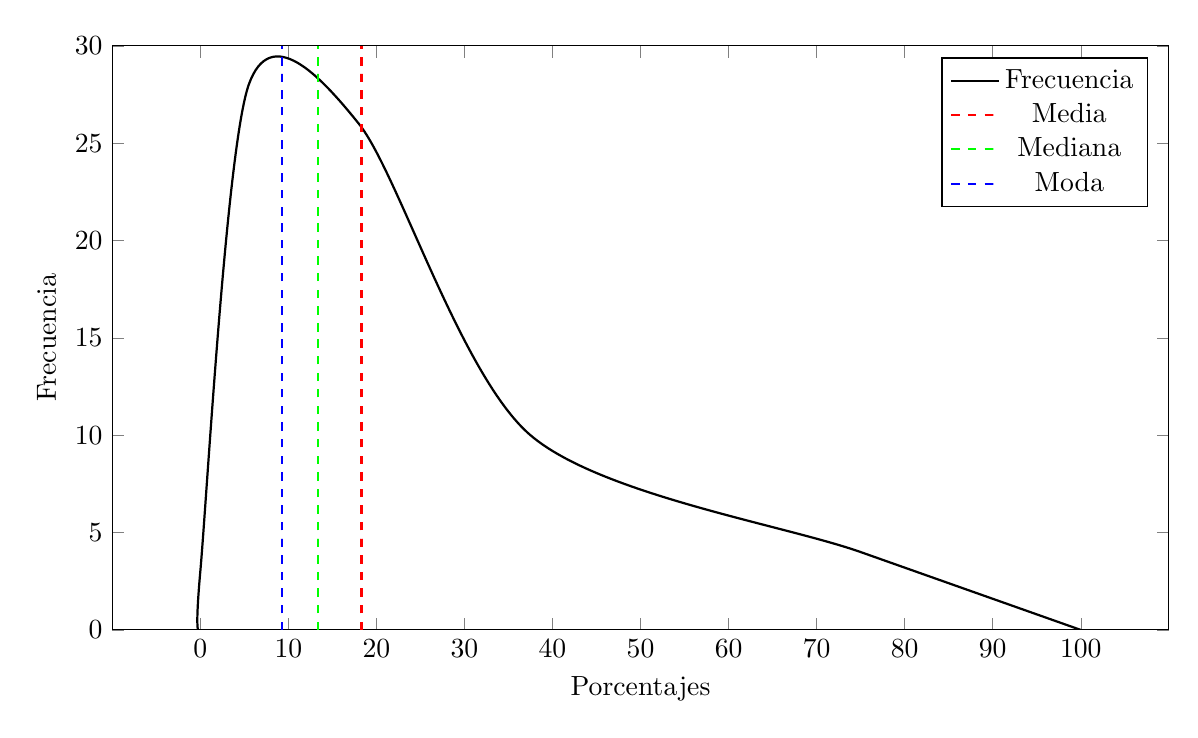
\begin{tikzpicture}
		\begin{axis}[
			width=15cm, height=9cm,
			xlabel={Porcentajes},
			ylabel={Frecuencia},
			xtick={0,10,20,30,40,50,60,70,80,90,100},
			ymin=0, ymax=30,
			grid=none,
			smooth,
			tension=0.5
			]
			\addplot[
			color=black,
			thick
			]coordinates{
				(0,0)
				(0,3)
				(5.5,28)
				(18,26)
				(37.5,10)
				(75,4)
				(100,0)
			};
			
			\addplot[
			color=red,
			thick,
			dashed
			]coordinates{(18.3,0)(18.3,30)};
			
			\addplot[
			color=green,
			thick,
			dashed
			]coordinates{(13.4,0)(13.4,30)};
			
			\addplot[
			color=blue,
			thick,
			dashed
			]coordinates{(9.3,0)(9.3,30)};
			\legend{Frecuencia, Media, Mediana, Moda}
		\end{axis}
	\end{tikzpicture}
	\caption{Distribución Positiva}
\end{figure}

\noindent\textbf{Interpretación de la información:}

Los resultados muestran que la mayoría de los participantes percibe un nivel bajo a moderado de automatización de tareas gracias a la IA, con el 38.89\% estimando entre un 1\% y un 10\% de automatización y el 36.11\% entre un 11\% y un 25\%. La media del 18.27\% y la mediana de 13.42\% reflejan esta tendencia, y la ligera asimetría positiva (1.90) indica una mayor concentración de respuestas en los valores bajos, con pocos participantes reportando niveles elevados de automatización. La curtosis leptocúrtica (0.43) sugiere una concentración de respuestas cerca de la media, consolidando la observación de que la mayoría ve un impacto limitado de la IA en sus tareas. En conjunto, estos hallazgos sugieren una implementación de IA aún incipiente en este contexto, con mayor aplicación en tareas específicas y menores porcentajes de automatización.
  
  % Pregunta 16